\documentclass[11pt,a4paper]{article}
\usepackage[utf8]{inputenc}
\usepackage[margin=0.7in]{geometry}
\usepackage{graphicx}
\usepackage[english]{babel}
\usepackage[style=authoryear, backend=biber]{biblatex}
\usepackage{tabularx}
\usepackage{booktabs}
\usepackage{float}
\usepackage{xltabular}
\usepackage{enumitem}

\begin{document}

\begin{titlepage}
    \centering
    \vspace*{\vfill} 

    {\Large \textbf{UNIVERSITY OF COMPUTER STUDIES, YANGON}} \\[0.5cm]
    {\large 2025 - 2026 Academic Year} \\[0.3cm]
    {\large Semester - III} \\[0.3cm]
    {\large Fundamental Database Management Project} \\[1.5cm]
   
    
\includegraphics[width=0.2\textwidth]{ucsy-logo.png} \\[2cm]

    {\LARGE \textbf{UCSY Learning Management System}} \\[2.5cm]
    
    {\large Covered By} \\[0.3cm]
    {\large \textbf{Fundamental Database Management System (IS-201)}} \\[0.2cm]
    {\large Faculty of Information Science} \\[3.5cm]

    {\large University of Computer Studies, Yangon} \\[0.3cm]
    {\large Submitted By} \\[0.2cm]
    {\large Group No -  (Section - B)} \\[0.3cm]
    {\large March, 2026}
    \vspace*{\vfill} 
\end{titlepage}
\newpage

\pagenumbering{arabic}
\tableofcontents
\newpage

\begin{table}[h]
\centering
\renewcommand{\arraystretch}{1.5}
\begin{tabularx}{\textwidth}{|p{1.5cm}|X|p{3cm}|p{3cm}|}
\hline
\textbf{No.} & \textbf{Name} & \textbf{YKPT} & \textbf{Role} \\ \hline
1 & Aung Myint Myat & 23046 & Project Leader\\ \hline
2 & Aung Khant Kyaw & 23023 &  Designer \\ \hline
3 & Phyo Khant Kyaw & 23027 & Designer \\ \hline
4 & Min Khant Aung & 23036 & Designer \\ \hline
5 & Chan Myaw Htike & 23057 & SQL \\ \hline
6 & Ye Kyaw Swar & 23050 &  SQL \\ \hline
7 & Htet Thu Aung & 23019 & SQL \\ \hline
8 & Aung Oo Khant & 23031 & Documentation \\ \hline
9 & Nyan Linn Htet & 23016 & Doucmentation \\ \hline
\end{tabularx}
\caption{Project Group Members List}
\end{table}
\newpage

\section{Introduction}
\paragraph{\indent Education is a very important part of life for everyone. A good school needs a strong system to manage students, teachers, and classes. In the past, many schools used paper and pens to keep records. This old way is slow and makes it easy to lose information. Today, schools use digital systems to make everything faster and more organized. This project focuses on building a Learning Management System (LMS) for UCSY. By using this system, the university can easily store data about departments, courses, and student grades in one safe place.}
\subsection{Project Description}
\paragraph{\indent Learning Management System (LMS) is a comprehensive database application created to streamline the administrative and academic processes of the university. The system serves as a central hub where students can view their schedules, instructors can manage their courses, and administrators can monitor the overall progress of the academic year. By organizing data into specific categories like Departments, Terms, and Sections, the system ensures a smooth flow of information across the campus.}

\paragraph{\textbf{Key Features:}}
\begin{itemize}[noitemsep]
    \item \textbf{Student \& Parent Management:} Stores student details and connects them to their parent's contact information.
    \item \textbf{Course \& Lecture Tracking:} Organizes different courses, who teaches them, and which room the class is in.
    \item \textbf{Attendance System:} Records the time students arrive and leave their classes.
    \item \textbf{Academic Resources:} Allows instructors to share links to videos, slides, and textbooks with students.
    \item \textbf{Assessment \& Grading:} Tracks assignments, quizzes, and exams, and stores the final scores and feedback.
    \item \textbf{Announcement Board:} Helps teachers send important news and updates to their students quickly.
\end{itemize}
\paragraph{\indent By integrating modern technology, this system reduces the administrative burdens, eliminates delays and enhances the efficiency of university learning management.}
\newline
\paragraph{To get a copy of our project, you can do the following steps:}

\begin{enumerate}
\item \textbf{Clone the repository.}
\begin{verbatim}
git clone https://github.com/ammdevl/ucsy_lms_db.git
\end{verbatim}

\item \textbf{Navigate to the project.}
\begin{verbatim}
cd ucsy_lms_db
\end{verbatim}

\item \textbf{Follow project-specific instructions.}
\begin{verbatim}
Read README.md
\end{verbatim}
\end{enumerate}
\newpage

\subsection{Project Objectives}
\paragraph{The main goal of this project is to create a simple, reliable, and helpful Learning Management System for the university. The specific objectives are:}

\begin{enumerate}
    \item To store student and teacher records accurately in a digital database.
    \item To help students check their class schedules and room numbers easily.
    \item To provide a way for instructors to share learning materials like slides and videos.
    \item To automate the tracking of student attendance for every class.
    \item To make it easy for teachers to record grades and give feedback to students.
    \item To ensure that parents can be contacted easily if there is an emergency or update.
    \item To improve communication between teachers and students through digital announcements.
    \item To reduce the use of paper and prevent the loss of important school data.
\end{enumerate}
\newpage

\section{Database Design and Query Execution}
\vspace{1cm}
\subsection{Entity Relationship (ER) Diagram Drawn in StarUML}
\vspace{2cm}
\begin{figure}[h]
    \centering
    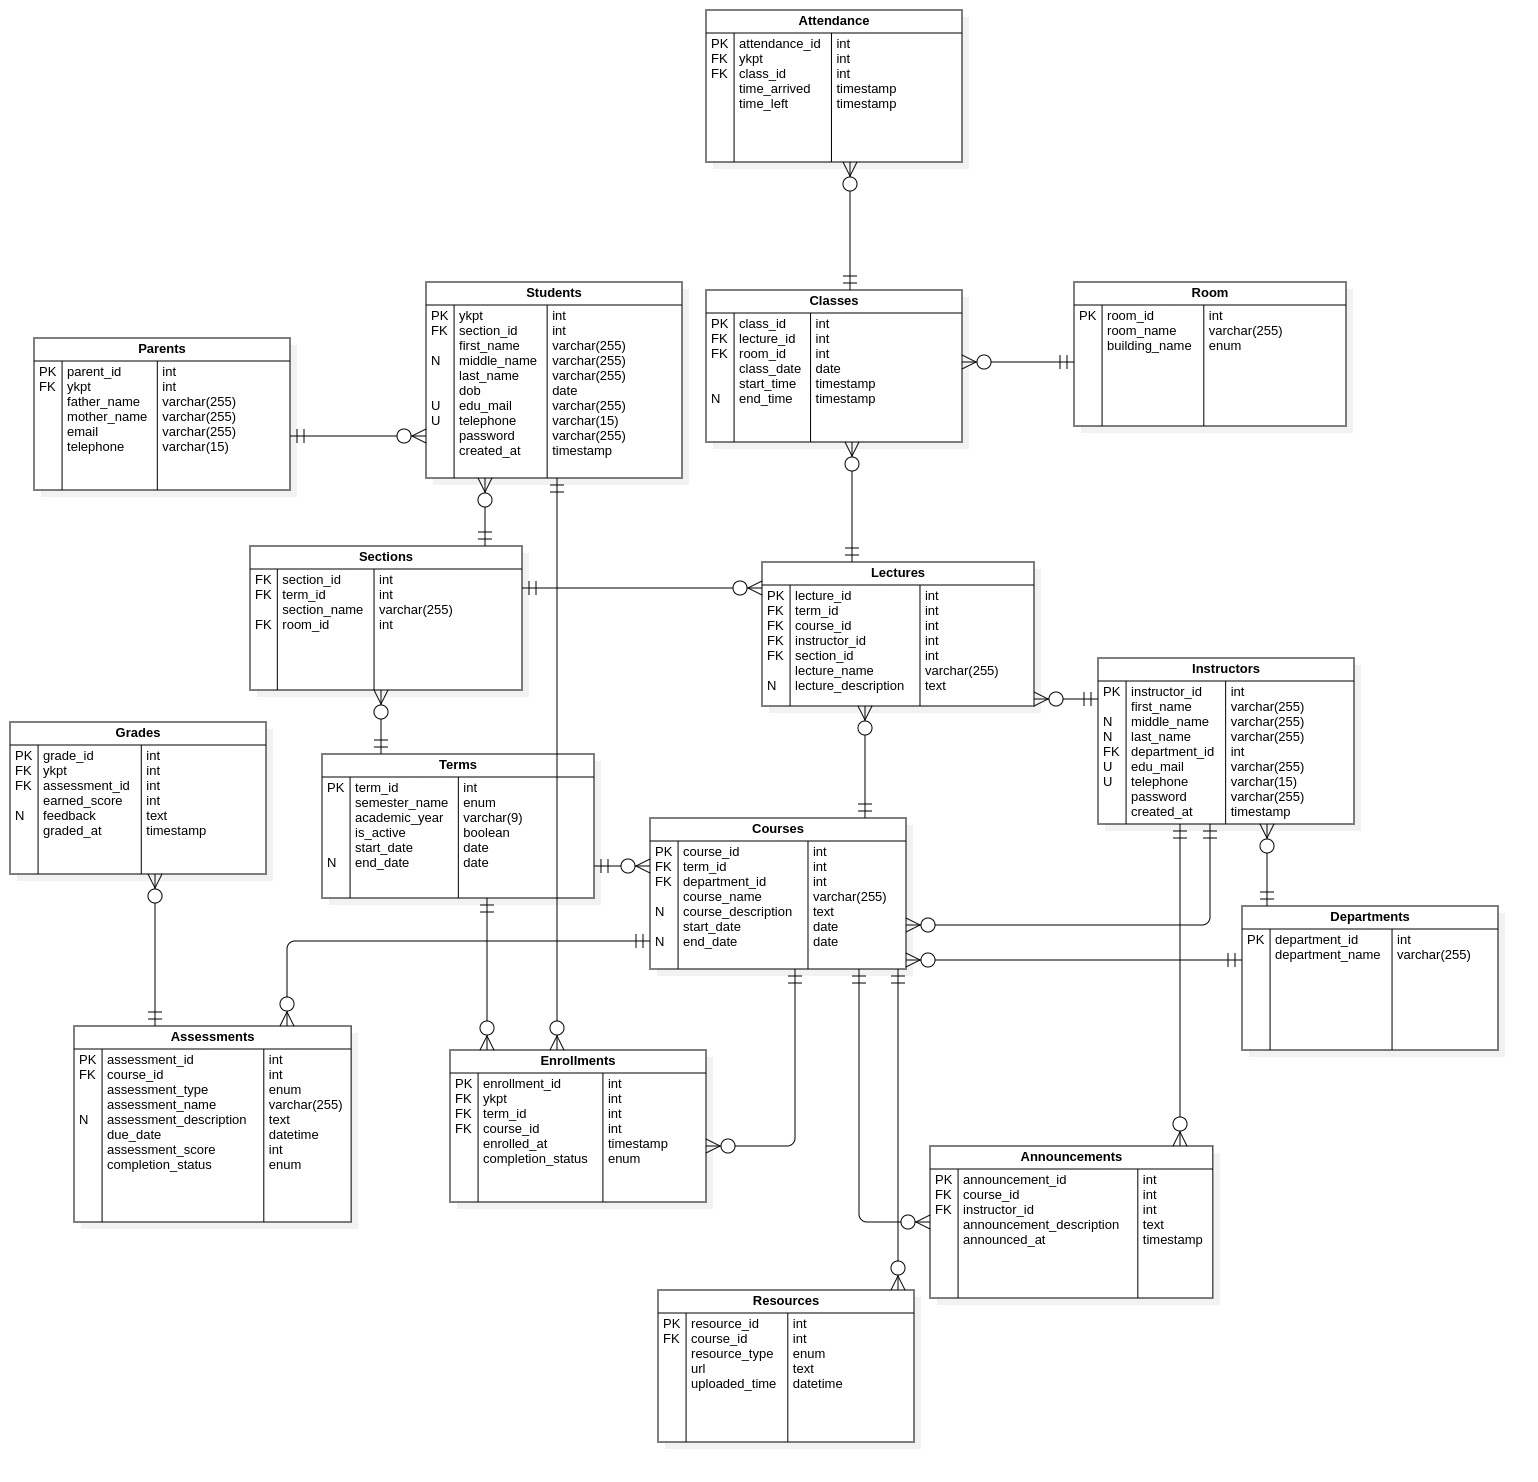
\includegraphics[width=\textwidth]{ucsy_lms_db_erd_staruml.png}
    \caption{E-R Diagram for UCSY LMS Drawn in StarUML}
\end{figure}
\newpage

\vspace{1cm}
\subsection{Entity Relationship (ER) Diagram Generated in MySQL Workbench}
\vspace{5cm}
\begin{figure}[h]
    \centering
    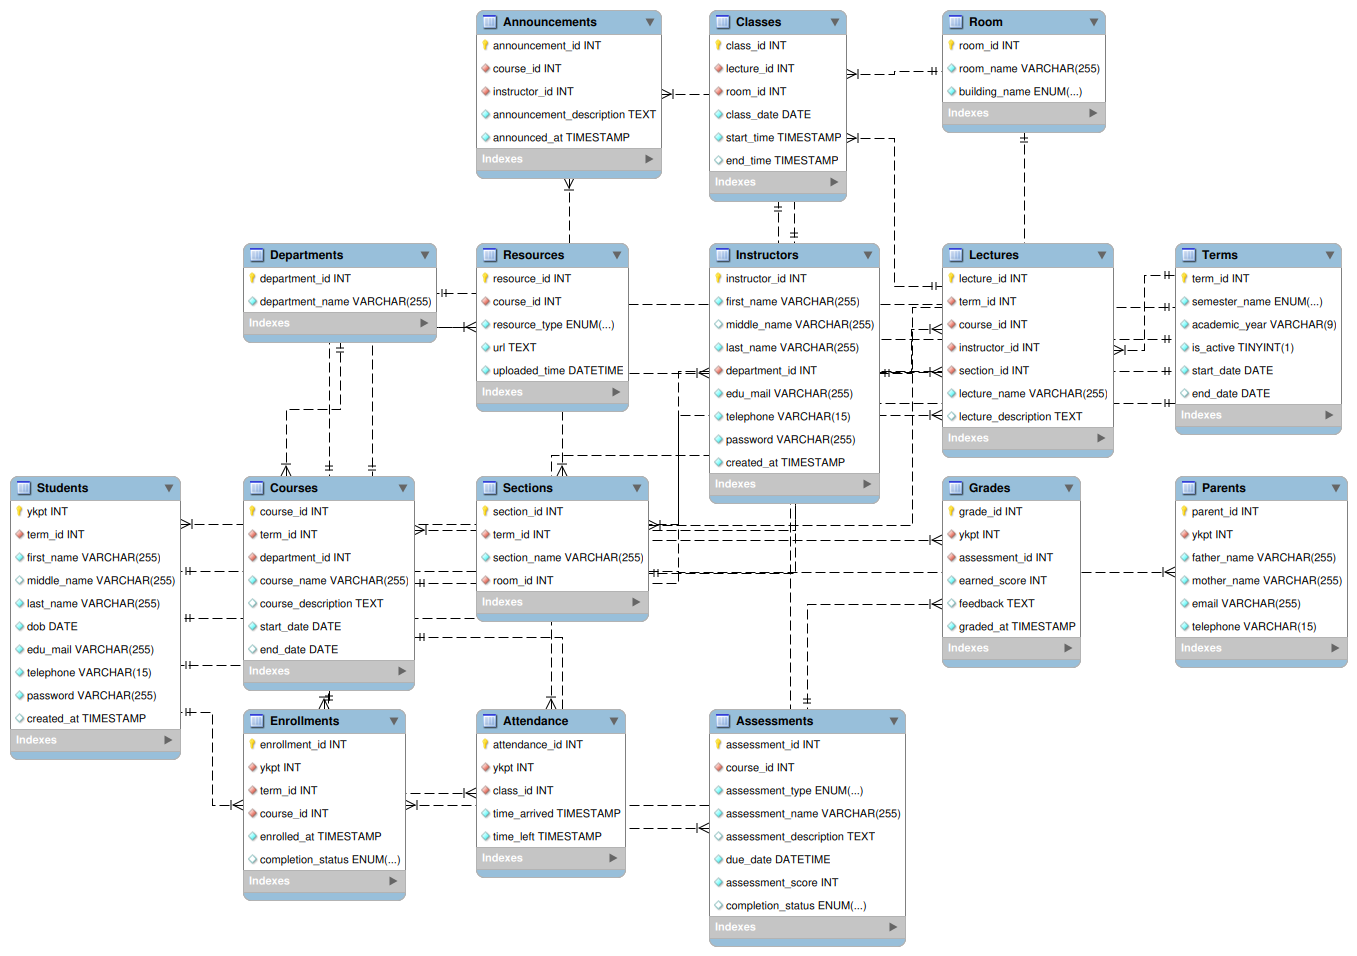
\includegraphics[width=\textwidth]{ucsy_lms_db_erd_mysql.png}
    \caption{E-R Diagram for UCSY LMS Generated in MySQL Workbench}
\end{figure}
\newpage

\subsection{Data Dictionary}
\begin{xltabular}{\textwidth}{|l|l|l|X|l|l|l|}
    \hline
    \textbf{Table} & \textbf{Field} & \textbf{Type} & \textbf{Description} & \textbf{Null} & \textbf{Key} & \textbf{Ref} \\ \hline
    \endfirsthead

    \hline
    \multicolumn{7}{|c|}{Continuation of Data Dictionary} \\
    \hline
    \textbf{Table} & \textbf{Field} & \textbf{Type} & \textbf{Description} & \textbf{Null} & \textbf{Key} & \textbf{Ref} \\ \hline
    \endhead

    \hline
    \multicolumn{7}{r}{Continued on next page...} \\
    \endfoot

    \hline
    \caption{Data Dictionary for ucsy\_lms\_db} \label{tab:database_schema}
    \endlastfoot

    % Departments
    Departments & department\_id & int & Unique ID for department & No & PK & \\ \hline
     & department\_name & varchar(255) & Department name & No & & \\ \hline
    
    % Room
    Room & room\_id & int & Unique ID for room & No & PK & \\ \hline
     & room\_name & varchar(255) & Name of the room & No & & \\ \hline
     & building\_name & enum & Building (A-F, Ext1-2) & No & & \\ \hline

    % Terms
    Terms & term\_id & int & Unique ID for term & No & PK & \\ \hline
     & semester\_name & enum & Semester (I to X) & No & & \\ \hline
     & academic\_year & varchar(9) & Academic year format & No & & \\ \hline
     & is\_active & boolean & Current active term status & No & & \\ \hline
     & start\_date & date & Term start date & No & & \\ \hline
     & end\_date & date & Term end date & Yes & & \\ \hline

    % Sections
    Sections & section\_id & int & Unique ID for section & No & PK & \\ \hline
     & term\_id & int & Reference to term & No & FK & Terms \\ \hline
     & section\_name & varchar(255) & Name of section & No & & \\ \hline
     & room\_id & int & Reference to room & No & FK & Room \\ \hline

    % Students
    Students & ykpt & int & Unique Student ID & No & PK & \\ \hline
     & term\_id & int & Reference to term & No & FK & Sections \\ \hline
     & first\_name & varchar(255) & First name & No & & \\ \hline
     & middle\_name & varchar(255) & Middle name & Yes & & \\ \hline
     & last\_name & varchar(255) & Last name & No & & \\ \hline
     & dob & date & Date of Birth & No & & \\ \hline
     & edu\_mail & varchar(255) & University email & No & & \\ \hline
     & telephone & varchar(15) & Phone number & No & & \\ \hline
     & password & varchar(255) & Hashed password & No & & \\ \hline
     & created\_at & timestamp & Record creation time & No & & \\ \hline

    % Parents
    Parents & parent\_id & int & Unique ID for parent & No & PK & \\ \hline
     & ykpt & int & Reference to student & No & FK & Students \\ \hline
     & father\_name & varchar(255) & Father's name & No & & \\ \hline
     & mother\_name & varchar(255) & Mother's name & No & & \\ \hline
     & email & varchar(255) & Contact email & No & & \\ \hline
     & telephone & varchar(15) & Contact phone & No & & \\ \hline

    % Instructors
    Instructors & instructor\_id & int & Unique ID for instructor & No & PK & \\ \hline
     & first\_name & varchar(255) & First name & No & & \\ \hline
     & middle\_name & varchar(255) & Middle name & Yes & & \\ \hline
     & last\_name & varchar(255) & Last name & No & & \\ \hline
     & department\_id & int & Reference to department & No & FK & Departments \\ \hline
     & edu\_mail & varchar(255) & Instructor email & No & & \\ \hline
     & telephone & varchar(255) & Phone number & No & & \\ \hline
     & password & varchar(255) & Hashed password & No & & \\ \hline

    % Courses
    Courses & course\_id & int & Unique ID for course & No & PK & \\ \hline
    	 & term\_id & int & Reference to term & No & FK & Terms \\ \hline
     & department\_id & int & Owning department & No & FK & Departments \\ \hline
     & course\_name & varchar(255) & Name of the course & No & & \\ \hline
     & course\_description & text & Course syllabus/info & Yes & & \\ \hline
     & start\_date & date & Commencement date & No & & \\ \hline
     & end\_date & date & Conclusion date & Yes & & \\ \hline

    % Lectures
    Lectures & lecture\_id & int & Unique ID for lecture & No & PK & \\ \hline
     & term\_id & int & Reference to term & No & FK & Terms \\ \hline
     & course\_id & int & Reference to course & No & FK & Courses \\ \hline
     & instructor\_id & int & Assigned instructor & No & FK & Instructors \\ \hline
     & section\_id & int & Assigned section & No & FK & Sections \\ \hline
     & lecture\_name & varchar(255) & Title of lecture & No & & \\ \hline
     & lecture\_description & text & Detailed info & Yes & & \\ \hline

    % Classes
    Classes & class\_id & int & Unique ID for class instance & No & PK & \\ \hline
     & lecture\_id & int & Reference to lecture & No & FK & Lectures \\ \hline
     & room\_id & int & Reference to room & No & FK & Room \\ \hline
     & class\_date & date & Date of the class & No & & \\ \hline
     & start\_time & timestamp & Scheduled start & No & & \\ \hline
     & end\_time & timestamp & Scheduled end & Yes & & \\ \hline

    % Enrollments
    Enrollments & enrollment\_id & int & Unique ID for enrollment & No & PK & \\ \hline
     & ykpt & int & Reference to student & No & FK & Students \\ \hline
     & term\_id & int & Reference to term & No & FK & Terms \\ \hline
     & course\_id & int & Reference to course & No & FK & Courses \\ \hline
     & enrolled\_at & timestamp & Time of enrollment & No & & \\ \hline
     & completion\_status & enum & Not Started/Progress/Done & No & & \\ \hline

    % Assessments
    Assessments & assessment\_id & int & Unique ID for assessment & No & PK & \\ \hline
     & course\_id & int & Reference to course & No & FK & Courses \\ \hline
     & assessment\_type & enum & Tutorial/Quiz/Lab/etc. & No & & \\ \hline
     & assessment\_name & varchar(255) & Name of assessment & No & & \\ \hline
     & due\_date & datetime & Deadline & No & & \\ \hline
     & assessment\_score & int & Max possible points & No & & \\ \hline

    % Attendance
    Attendance & attendance\_id & int & Unique ID for attendance & No & PK & \\ \hline
     & ykpt & int & Reference to student & No & FK & Students \\ \hline
     & class\_id & int & Reference to class & No & FK & Classes \\ \hline
     & time\_arrived & timestamp & Arrival timestamp & No & & \\ \hline
     & time\_left & timestamp & Departure timestamp & No & & \\ \hline

    % Resources
    Resources & resource\_id & int & Unique ID for resource & No & PK & \\ \hline
     & course\_id & int & Reference to course & No & FK & Courses \\ \hline
     & resource\_type & enum & Video/Slides/Book/etc. & No & & \\ \hline
     & url & text & Link to resource & No & & \\ \hline
     & uploaded\_time & datetime & Time of upload & No & & \\ \hline

    % Grades
    Grades & grade\_id & int & Unique ID for grade & No & PK & \\ \hline
     & ykpt & int & Reference to student & No & FK & Students \\ \hline
     & assessment\_id & int & Reference to assessment & No & FK & Assessments \\ \hline
     & earned\_score & int & Actual points earned & No & & \\ \hline
     & feedback & text & Instructor comments & Yes & & \\ \hline
     & graded\_at & timestamp & Time of grading & No & & \\ \hline

    % Announcements
    Announcements & announcement\_id & int & Unique ID for post & No & PK & \\ \hline
     & course\_id & int & Reference to course & No & FK & Courses \\ \hline
     & instructor\_id & int & Reference to instructor & No & FK & Instructors \\ \hline
     & announcement\_description & text & Post content & No & & \\ \hline
     & announced\_at & timestamp & Time of post & No & & \\ \hline
\end{xltabular}
\newpage

\subsection{Data Insertion in Relational Tables}
\vspace{3cm}
\begin{figure}[h]
    \centering
    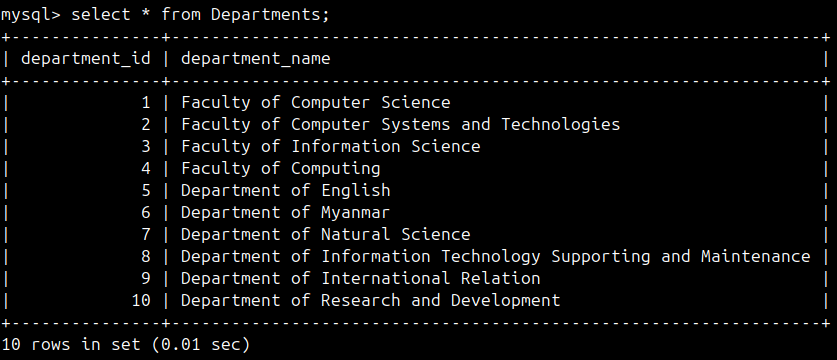
\includegraphics[width=\textwidth]{departments.png}
    \caption{Data Insertion in Departments Table}
\end{figure}
\begin{figure}[h]
    \centering
    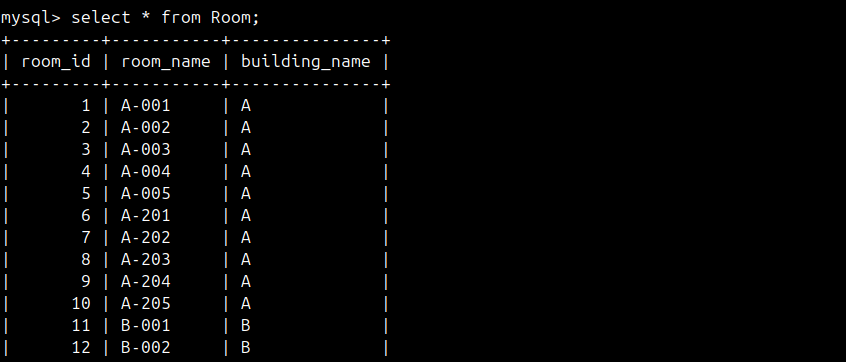
\includegraphics[width=\textwidth]{room.png}
    \caption{Data Insertion in Room Table}
\end{figure}
\newpage

\vspace{3cm}
\begin{figure}[h]
    \centering
    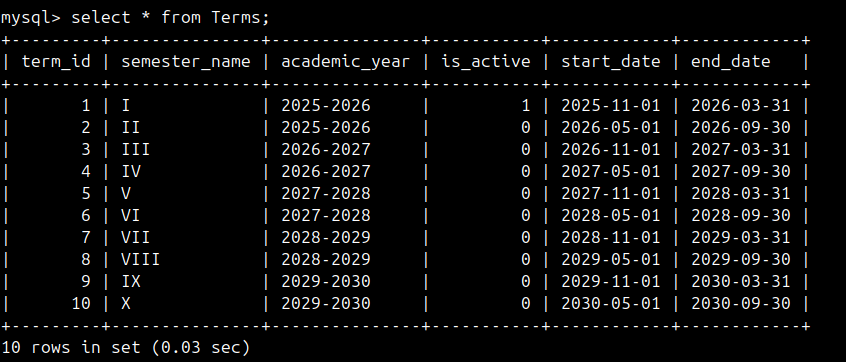
\includegraphics[width=\textwidth]{terms.png}
    \caption{Data Insertion in Terms Table}
\end{figure}
\begin{figure}[h]
    \centering
    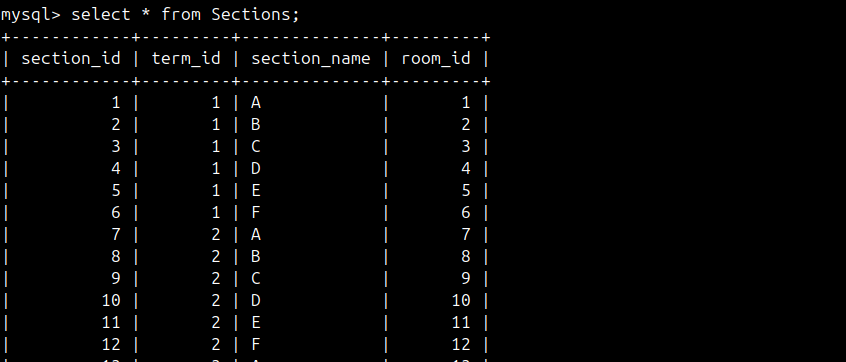
\includegraphics[width=\textwidth]{sections.png}
    \caption{Data Insertion in Sections Table}
\end{figure}
\newpage

\vspace{3cm}
\begin{figure}[h]
    \centering
    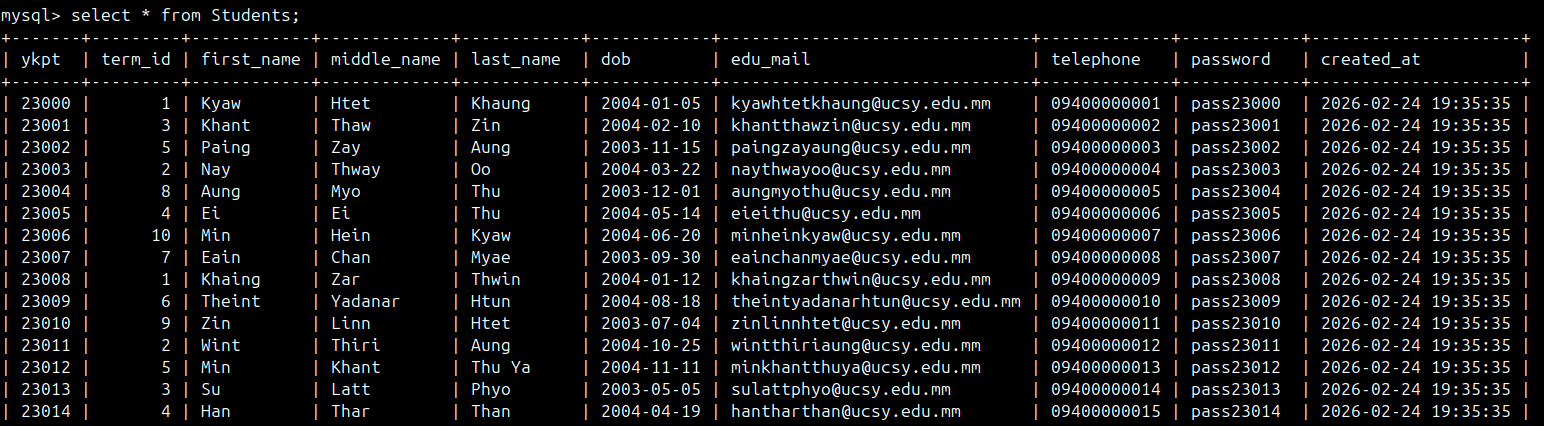
\includegraphics[width=\textwidth]{students.png}
    \caption{Data Insertion in Students Table}
\end{figure}
\begin{figure}[h]
    \centering
    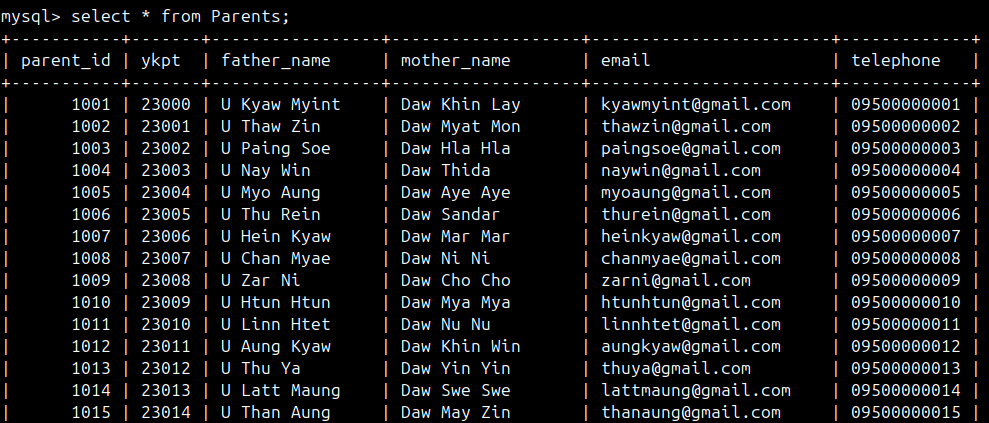
\includegraphics[width=\textwidth]{parents.png}
    \caption{Data Insertion in Parents Table}
\end{figure}
\newpage

\vspace{3cm}
\begin{figure}[h]
    \centering
    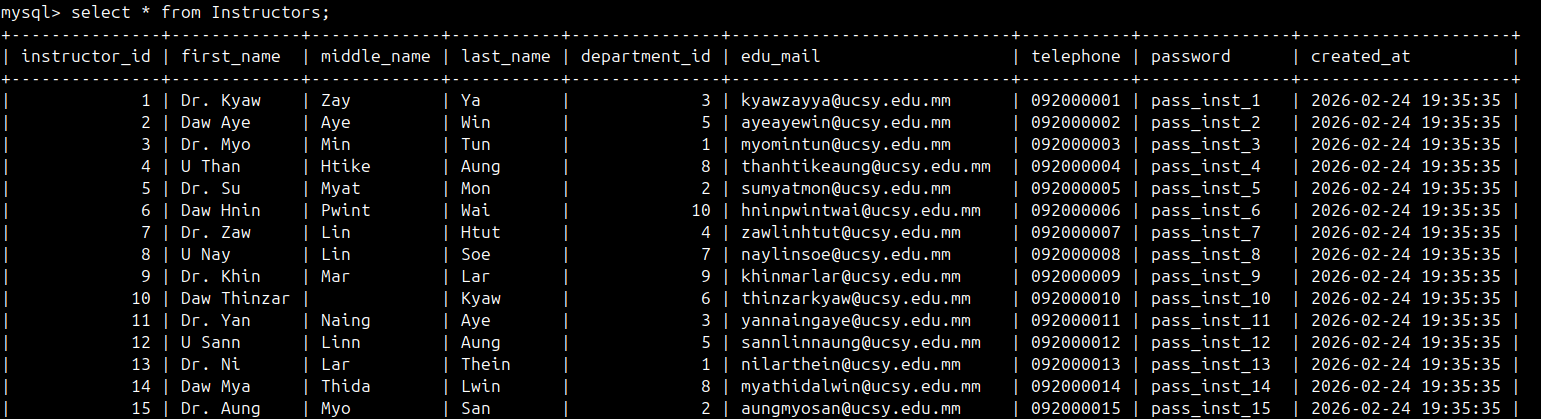
\includegraphics[width=\textwidth]{instructors.png}
    \caption{Data Insertion in Instructors Table}
\end{figure}
\begin{figure}[h]
    \centering
    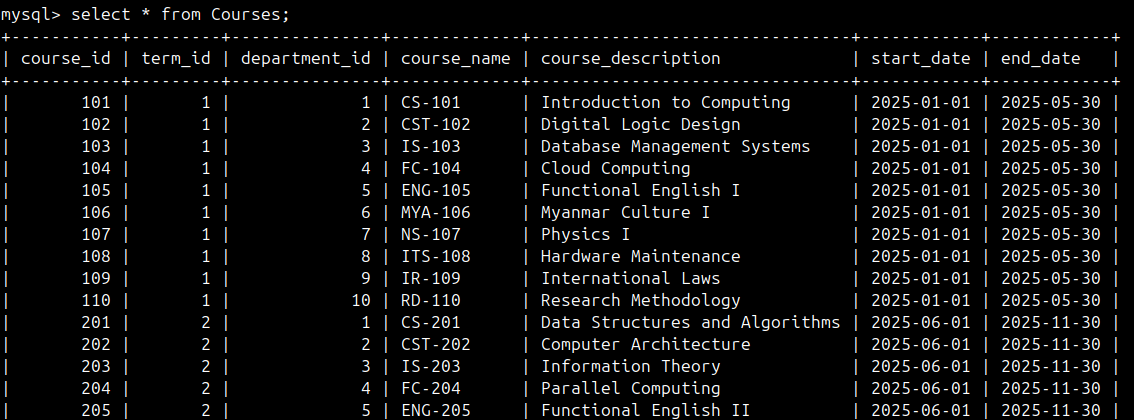
\includegraphics[width=\textwidth]{courses.png}
    \caption{Data Insertion in Courses Table}
\end{figure}
\newpage

\vspace{3cm}
\begin{figure}[h]
    \centering
    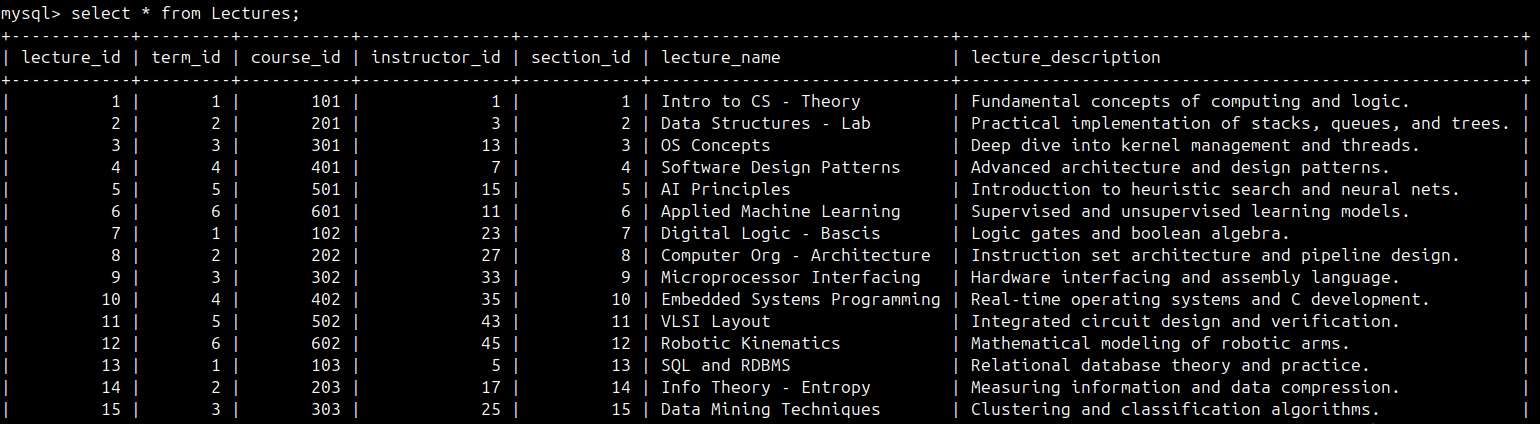
\includegraphics[width=\textwidth]{lectures.png}
    \caption{Data Insertion in Lectures Table}
\end{figure}
\begin{figure}[h]
    \centering
    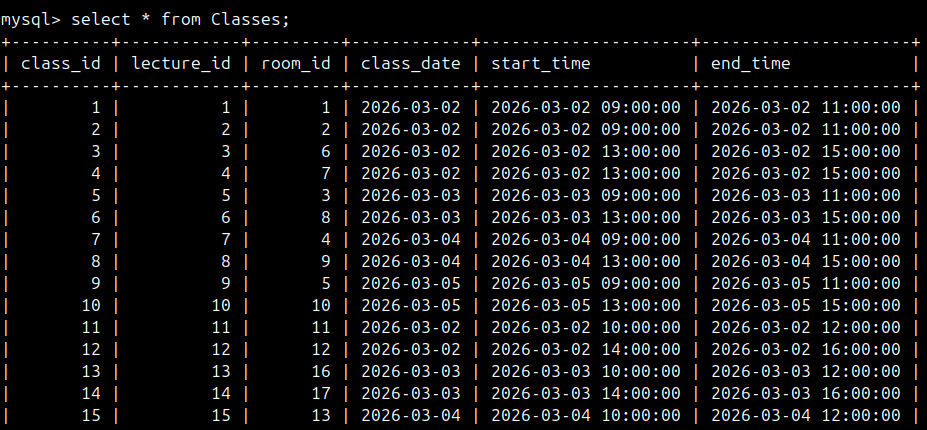
\includegraphics[width=\textwidth]{classes.png}
    \caption{Data Insertion in Classes Table}
\end{figure}
\newpage
\begin{figure}[h]
    \centering
    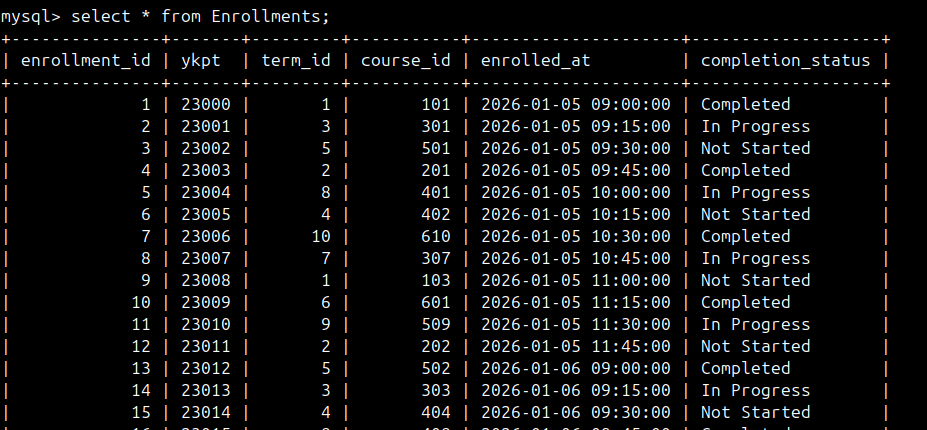
\includegraphics[width=\textwidth]{enrollments.png}
    \caption{Data Insertion in Enrollments Table}
\end{figure}
\begin{figure}[h]
    \centering
    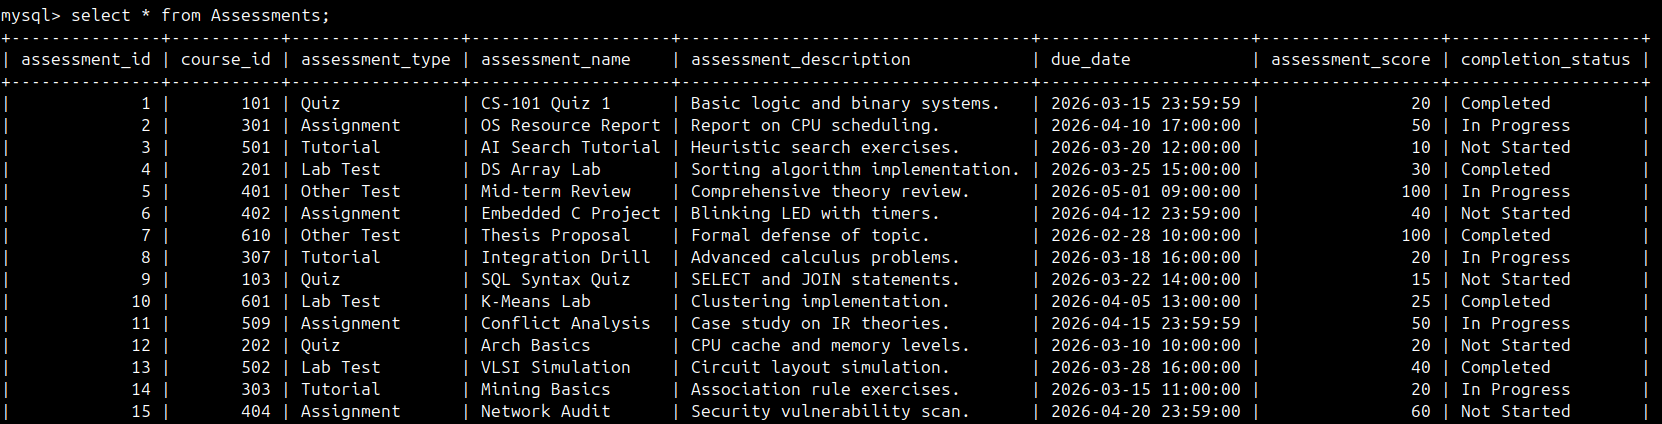
\includegraphics[width=\textwidth]{assessments.png}
    \caption{Data Insertion in Assessments Table}
\end{figure}
\newpage

\vspace{3cm}
\begin{figure}[h]
    \centering
    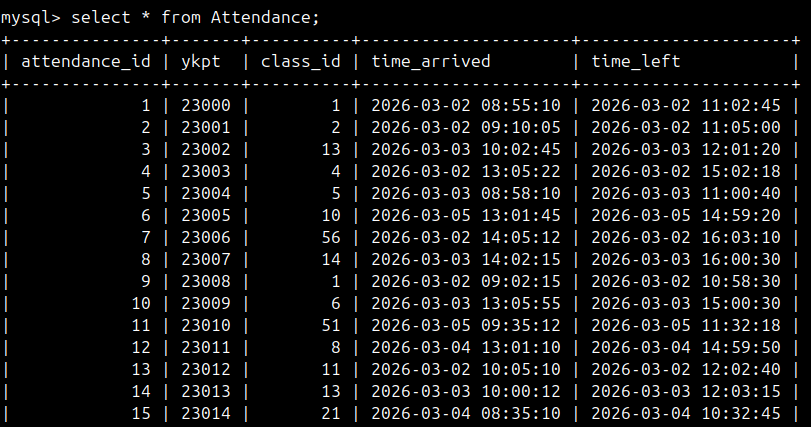
\includegraphics[width=\textwidth]{attendance.png}
    \caption{Data Insertion in Attendance Table}
\end{figure}
\begin{figure}[h]
    \centering
    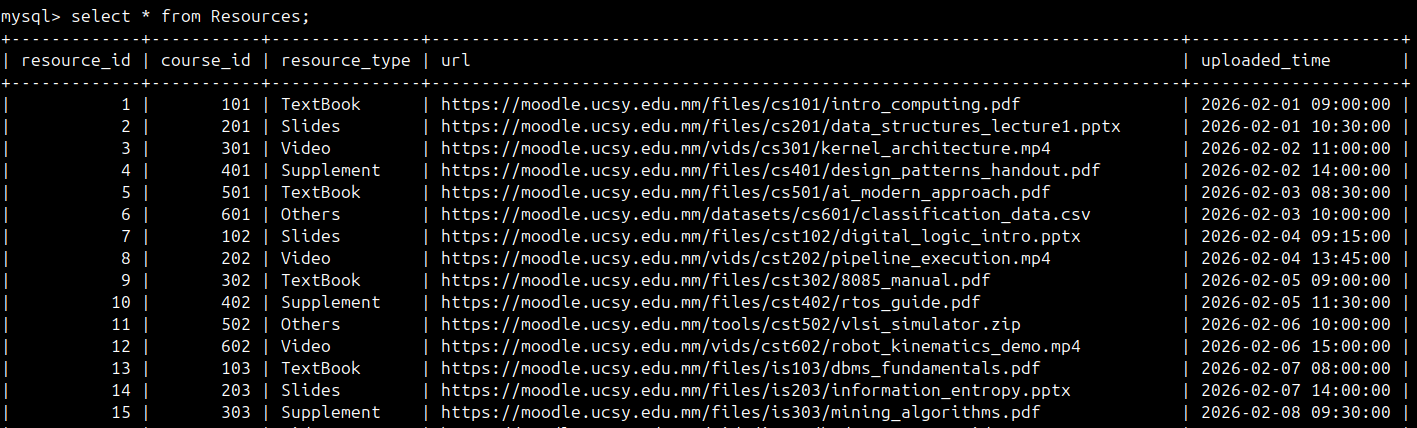
\includegraphics[width=\textwidth]{resources.png}
    \caption{Data Insertion in Resources Table}
\end{figure}
\newpage

\vspace{3cm}
\begin{figure}[h]
    \centering
    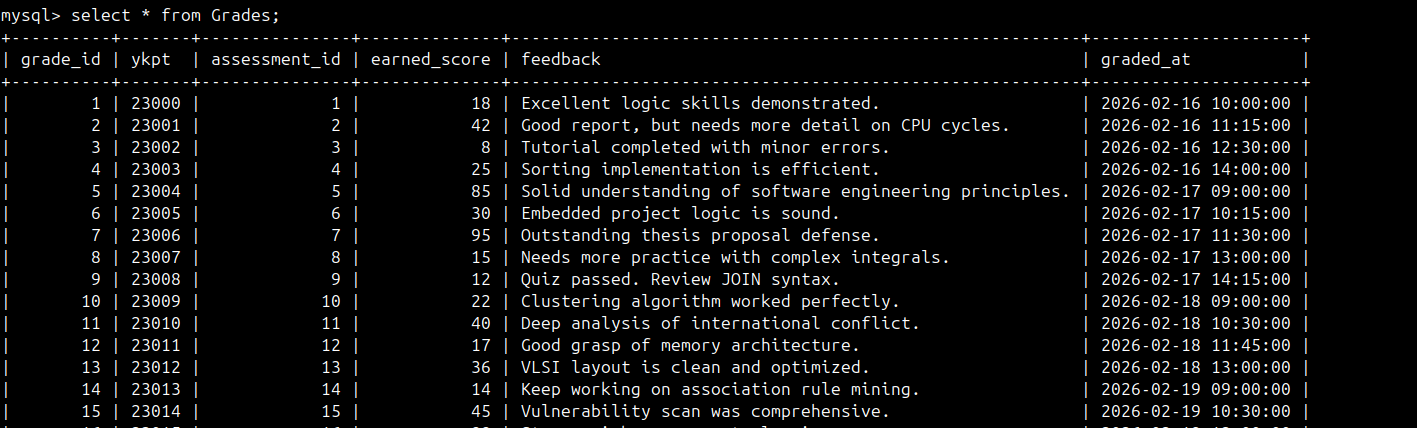
\includegraphics[width=\textwidth]{grades.png}
    \caption{Data Insertion in Grades able}
\end{figure}
\begin{figure}[h]
    \centering
    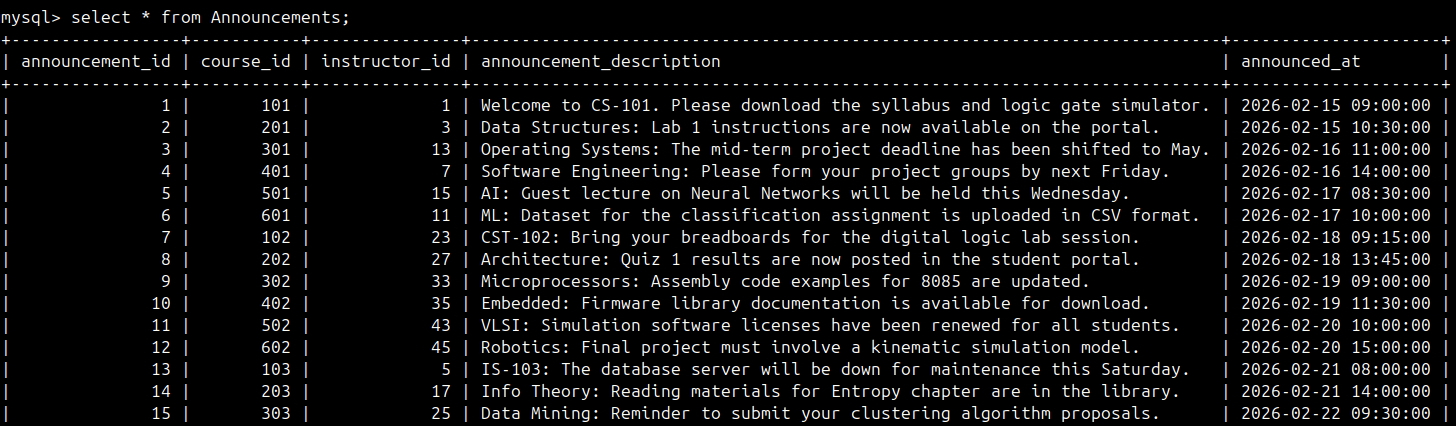
\includegraphics[width=\textwidth]{announcements.png}
    \caption{Data Insertion in Announcements Table}
\end{figure}
\newpage
\subsection{Client Requirements}
\begin{enumerate}
\item Find the total number of students enrolled in each department and sort by the highest number?
\item Check how many courses are currently "In Progress" for a specific term (e.g., 'Term 1')?
\item Find the number of late attendance records for each student?
\item Retrieve the instructor with the highest number of assigned lectures and their details?
\item Find all assessments that are past their due date and have not been completed?
\item Find all students who have a grade lower than 50 in "CS-101 Programming"?
\item How can I retrieve the full enrollment history of a specific student (e.g., Student ID 23023)?
\item What is the total number of resources available for a specific course (e.g., 'IS-103 Database')?
\end{enumerate}
\newline
\subsection{Query Planning with Algebra}
\begin{enumerate}[itemsep=1.5cm] % Added space to fill A4 page

\item Calculate the total number of students in each department and sort by highest enrollment?

$$\Pi_{\text{Department\_name, Total\_Students}}$$
$$(\gamma_{\text{Department\_name; COUNT(ykpt)}} (\text{Departments} \bowtie \text{Instructors} \bowtie \text{Lectures} \bowtie \text{Enrollments}))$$
$$\bowtie (\tau_{\text{Total\_Students DESC}})$$

\item How can I check how many courses are currently 'In Progress' for 'Term 1'?

$$\Pi_{\text{term\_id, In\_Progress\_Courses}}$$
$$(\gamma_{\text{term\_id; COUNT(course\_id)}} (\sigma_{\text{Completion\_status="In Progress" } \wedge \text{ term\_id=1}}(\text{Enrollments})))$$

\item Find the number of late attendance records for each student?

$$\Pi_{\text{ykpt, Late\_Count}}$$
$$(\gamma_{\text{ykpt; COUNT(attendance\_id)}} (\sigma_{\text{time\_arrived > expected\_start\_time}}(\text{Attendance})))$$

\item Retrieve the instructor with the highest number of assigned lectures and their details?

$$\Pi_{\text{instructor\_id, first\_name, last\_name, lecture\_count}}$$
$$(\sigma_{\text{lecture\_count} \ge (\text{MAX(lecture\_Count)}(\gamma_{\text{instructor\_id; lecture\_count := COUNT(lecture\_id)}}(\text{instructors} \bowtie \text{Lectures})))))$$

\item Find all assessments that are past their due date and have not been completed?

$$\Pi_{\text{assessment\_name, due\_date, course\_id}}$$
$$(\sigma_{\text{completion\_status='Not Started'} \wedge \text{ due\_date < CURRENT\_DATE}}(\text{Assessments}))$$

\item How can I retrieve the enrollment history of a specific student (e.g., Student ID 23023)?

$$\Pi_{\text{ykpt, course\_name, completion\_status}}$$
$$(\sigma_{\text{ykpt = 23023}}(\text{Enrollments} \bowtie \text{Courses}))$$

\item What is the total number of resources available for 'IS-103 Database'?

$$\Pi_{\text{course\_name, total\_Resources}}$$
$$(\sigma_{\text{course\_name = 'IS-103 Database'}}) (\gamma_{\text{course\_name; SUM(1)} \to \text{Total\_Resources}}(\text{Courses} \bowtie \text{Resources}))$$

\end{enumerate}
\newpage

\subsection{Query Execution with MySQL}
1. Find the total number of students enrolled in each department and sort by highest enrollment?
\begin{figure}[h]
    \centering
    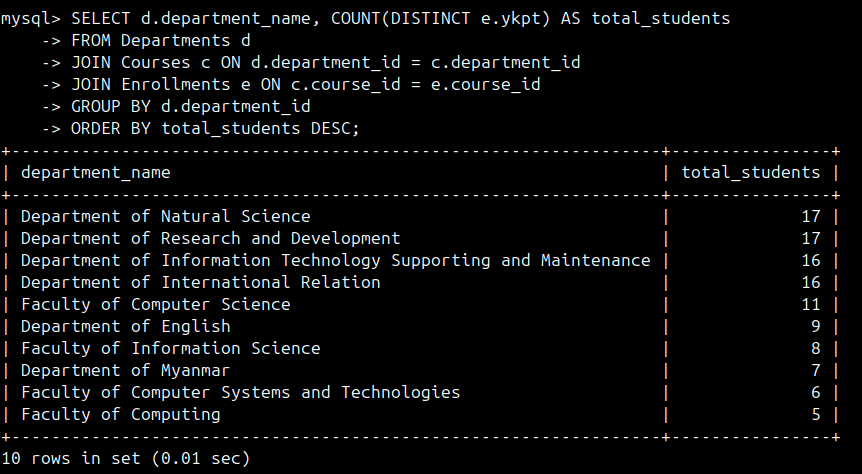
\includegraphics[width=\textwidth]{query1.png}
    \caption{Query for Question No. 1}
\end{figure}

2. Check how many courses are currently 'In Progress' for 'Term 1'?
\begin{figure}[h]
    \centering
    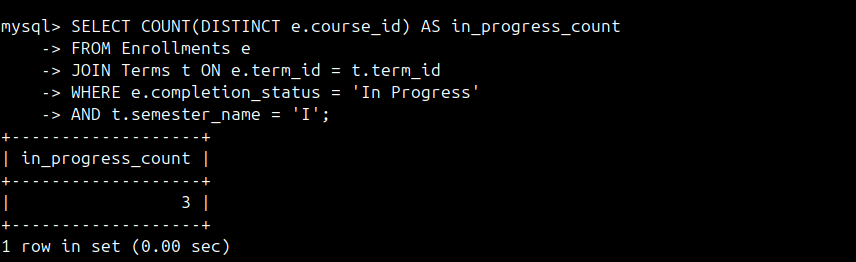
\includegraphics[width=\textwidth]{query2.png}
    \caption{Query for Question No. 2}
\end{figure}
\newpage

3. Find the number of late attendance records for each student?
\begin{figure}[h]
    \centering
    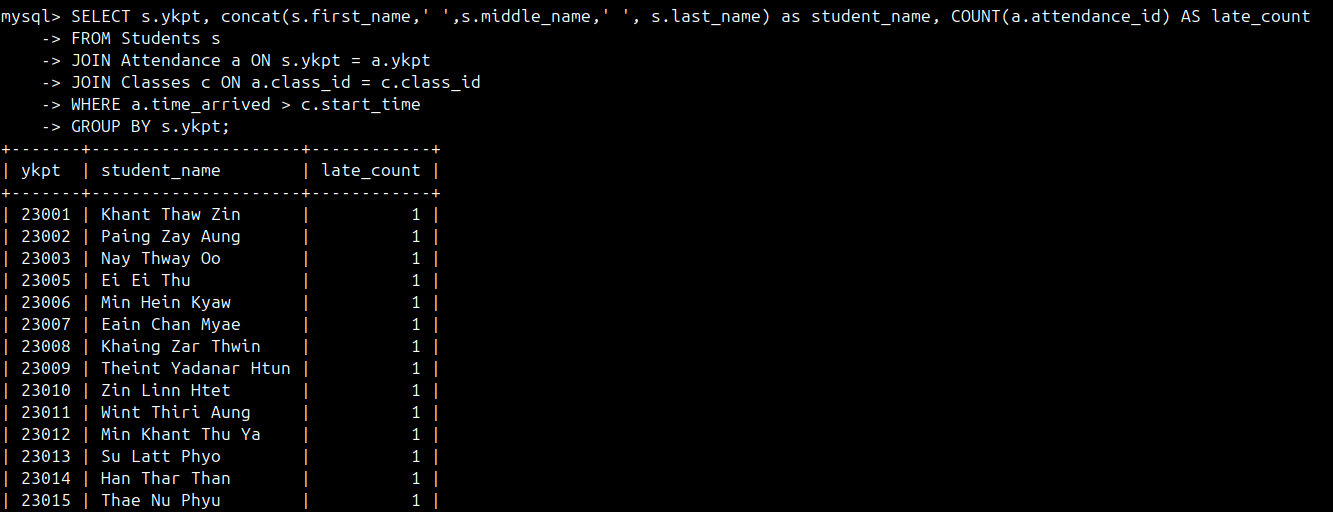
\includegraphics[width=\textwidth]{query3.png}
    \caption{Query for Question No. 3}
\end{figure}


4. Retrieve the instructor with the highest number of assigned lectures and their details?
\begin{figure}[h]
    \centering
    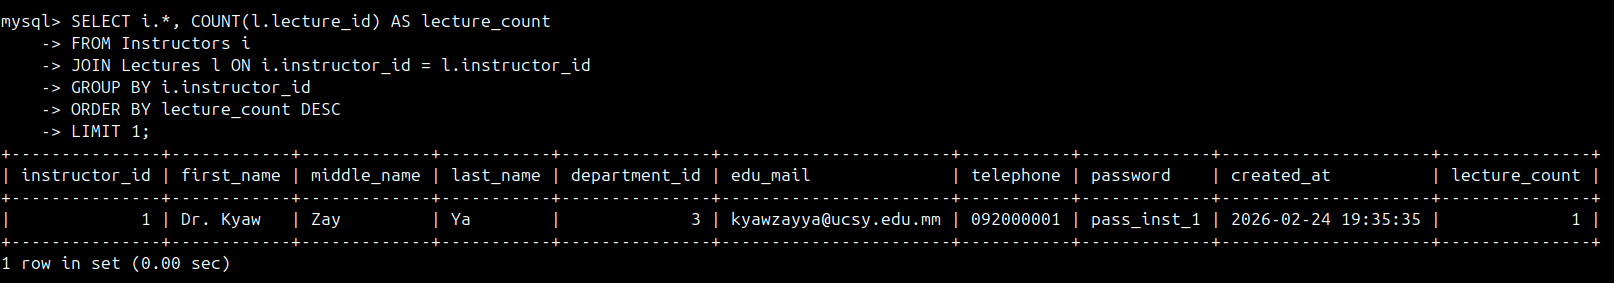
\includegraphics[width=\textwidth]{query4.png}
    \caption{Query for Question No. 4}
\end{figure}
\newpage

5. Find all assessments that are past their due date and have not been completed?
\begin{figure}[h]
    \centering
    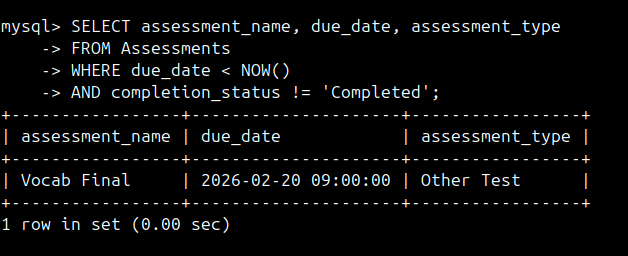
\includegraphics[width=\textwidth]{query5.png}
    \caption{Query for Question No. 5}
\end{figure}

6. Retrieve the enrollment history and completion status for a specific student (ID: 23023)?
\begin{figure}[h]
    \centering
    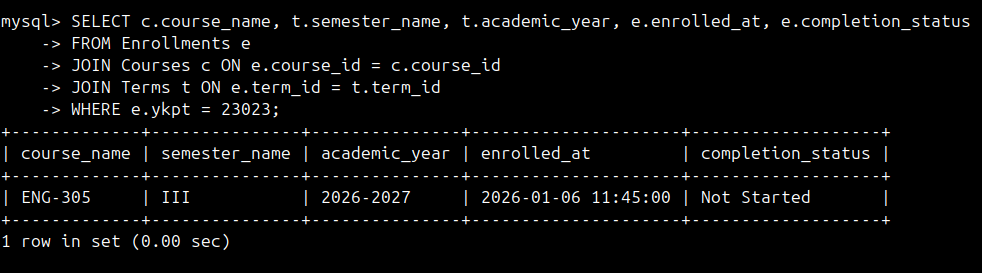
\includegraphics[width=\textwidth]{query6.png}
    \caption{Query for Question No. 6}
\end{figure}
\newpage

7. What is the total number of academic resources available for the 'CS-101' course?
\begin{figure}[h]
    \centering
    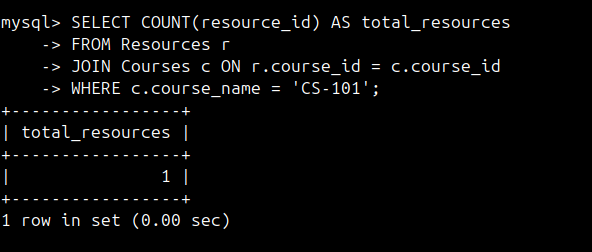
\includegraphics[width=\textwidth]{query7.png}
    \caption{Query for Question No. 7}
\end{figure}

8. Identify students who have attended a specific class (Class ID: 1) and their arrival times?
\begin{figure}[h]
    \centering
    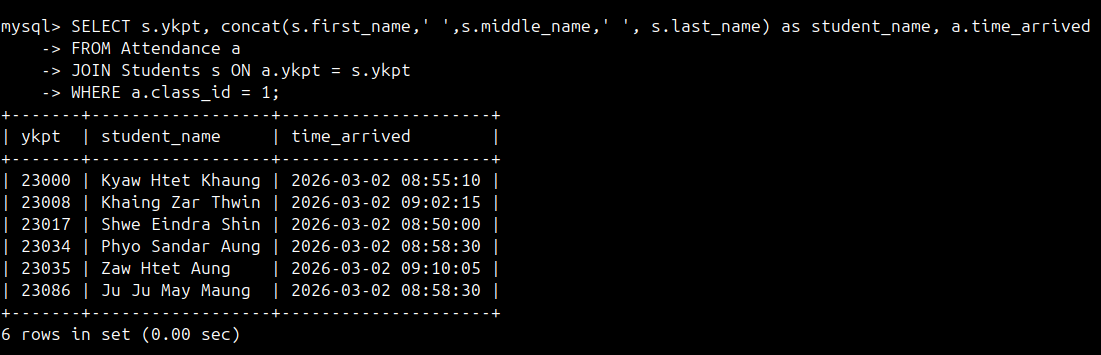
\includegraphics[width=\textwidth]{query8.png}
    \caption{Query for Question No. 8}
\end{figure}
\newpage

\section{Conclusion}
\paragraph{\indent The UCSY Learning Management System (LMS) successfully addresses the challenges of managing a modern university's academic operations. By replacing traditional, manual record-keeping with a centralized digital database, the university can now ensure that all information regarding students, instructors, and courses is accurate, secure, and easily accessible. This system streamlines the most essential university tasks, including student enrollment, classroom scheduling, attendance tracking, and grading, on a single, user-friendly platform. Students can now access their learning materials, such as slides and video tutorials, at any time, which promotes a more flexible and modern learning environment. Additionally, the integrated attendance and assessment modules provide instructors with real-time data to monitor student progress and provide immediate feedback, ensuring a high standard of education. Furthermore, the system strengthens the communication link between the university, its faculty, and the students' families. By maintaining secure records of parent contact information and offering a digital announcement board, the university can share urgent updates instantly, reducing administrative delays. The use of modern technology not only eliminates manual errors and potential fraud but also significantly reduces the burden on university staff.In summary, the UCSY Learning Management System plays a vital role in digitizing the campus. By reducing paper use and enhancing institutional coordination, the system provides a foundation for a more efficient, transparent, and organized academic future. It is a powerful tool that helps the University of Computer Studies, Yangon, provide a better and more professional experience for every student and teacher.}
\newpage

\begin{appendix}
	\section{Appendix}
	\listoftables
	\listoffigures
	\section{REFERENCES}
	\paragraph{• Mastering Database Design: An Ultimate Guide - GeeksforGeeks}
	\begin{verbatim}
		https://www.geeksforgeeks.org/dbms/database-design-ultimate-guide/
	\end{verbatim}
	\paragraph{• 7 Useful Database Diagram Examples | Redgate}
	\begin{verbatim}
		https://www.red-gate.com/blog/database-diagrams-examples
	\end{verbatim}
\end{appendix}

\end{document}
